\section{Experimental Results and Performance Analysis}
\label{sec:results}

This section presents the empirical benchmark results gathered across our primary Linux testbed. All quantitative values originate from the verified primary dataset in the project repository (\path{results/unified/processed/statistical_summary.csv}).

\subsection{Round-Trip Latency and Throughput Scaling}
Table~\ref{tab:benchmark_results} summarizes the mean round-trip latency ($\mu\text{s}$) across all seven payload classes, and Fig.~\ref{fig:latency_throughput} depicts round-trip latency and bandwidth scaling side-by-side on logarithmic axes.

\begin{figure*}[!t]
\centering
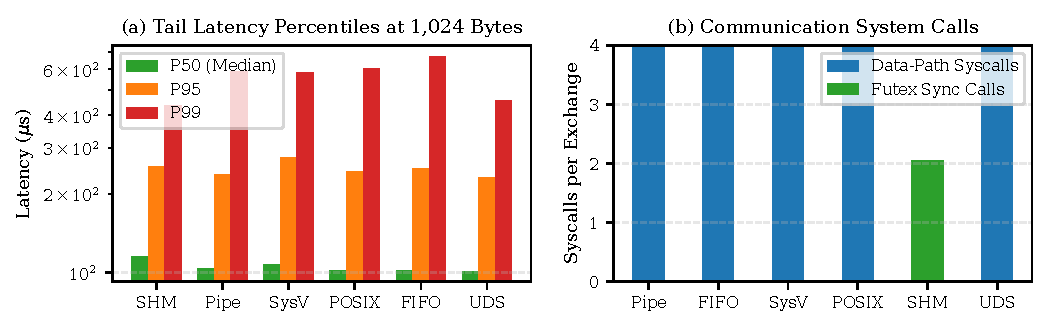
\includegraphics[height=4.2cm]{figures/percentiles_resources_combined.pdf}
\caption{Tail Latency and Operating System Resource Profiling on Fedora 45 Linux: (a) Median ($P_{50}$) and Tail Percentiles ($P_{95}, P_{99}$) for 1,024-Byte Payloads (logarithmic scale), and (b) Classified Communication System Calls per Round-Trip Exchange.}
\label{fig:percentiles_resources}
\end{figure*}

The latency data reveals three clear performance regimes:
\textbf{1) Sub-Kilobyte Regime ($\le 256$~B):} POSIX Shared Memory achieves the lowest round-trip latency among all userspace mechanisms ($286.87\,\mu\text{s}$ at 64~B and $320.35\,\mu\text{s}$ at 256~B). Because memory writes execute directly in userspace without entering the Linux VFS or network stack, SHM outperforms Anonymous Pipes by 28.1\% at 64~B ($286.87\,\mu\text{s}$ vs. $399.25\,\mu\text{s}$) and Named FIFOs by 38.2\% ($464.27\,\mu\text{s}$).
\textbf{2) Intermediate Regime (1~KB to 64~KB):} Anonymous Pipes deliver the lowest round-trip latency ($278.76\,\mu\text{s}$ at 1~KB and $301.70\,\mu\text{s}$ at 4~KB). At 1,024~bytes, Anonymous Pipes surpass POSIX Shared Memory ($351.15\,\mu\text{s}$) by 20.6\%. This occurs because the Linux pipe circular buffer (defaulting to 64~KB) absorbs 1~KB and 4~KB writes without blocking, whereas POSIX semaphores incur userspace-to-kernel transition penalties under lockstep ping-pong coordination.
\textbf{3) Large Payload Regime (256~KB):} For 262,144-byte transfers, Unix Domain Sockets achieve superior performance ($2,590.28\,\mu\text{s}$), outperforming Anonymous Pipes ($4,548.77\,\mu\text{s}$) by \textbf{1.756$\times$} and Named FIFOs ($4,217.02\,\mu\text{s}$) by 1.628$\times$. Because standard pipes default to a 64~KB capacity, transferring 256~KB forces four sequential chunked writes and reads, triggering multiple blocking context switches. Conversely, Unix domain stream sockets dynamically expand their socket buffers (\texttt{sk\_buff}), absorbing large payloads with fewer scheduling interruptions.

Throughput analysis (Fig.~\ref{fig:latency_throughput}(b)) confirms these crossover dynamics: for 64~B messages, POSIX Shared Memory achieves 3,485.90~msg/s ($0.343$~MB/s), followed by System V MQ at 2,780.94~msg/s ($0.279$~MB/s) and Anonymous Pipes at 2,504.70~msg/s ($0.321$~MB/s). At 64~KB, Anonymous Pipes reach their peak bandwidth of \textbf{241.29~MB/s} ($3,860.60$~msg/s). At 256~KB, Unix Domain Sockets dominate the evaluation spectrum, sustaining \textbf{167.84~MB/s} ($671.34$~msg/s), whereas pipe bandwidth collapses to 73.54~MB/s due to buffer exhaustion.

\subsection{Tail-Latency Distribution and Resource Profiling}
Tail latencies dictate real-time deadlines and predictable service-level objectives (SLOs). Fig.~\ref{fig:percentiles_resources}(a) displays the median ($P_{50}$) and tail percentiles ($P_{95}, P_{99}$) for 1,024-byte payloads, while Fig.~\ref{fig:percentiles_resources}(b) summarizes classified system calls per exchange.

The percentile analysis exposes severe tail degradation in file-backed and socket mechanisms:
\begin{itemize}[leftmargin=*,noitemsep,topsep=1.5pt]
    \item \textbf{Anonymous Pipes:} Lowest median latency ($P_{50} = 119.34\,\mu\text{s}$) and tightly bound tails ($P_{95} = 255.20\,\mu\text{s}$, $P_{99} = 392.06\,\mu\text{s}$).
    \item \textbf{POSIX Shared Memory:} Excellent median performance ($P_{50} = 154.21\,\mu\text{s}$) and compact $P_{95}$ ($786.76\,\mu\text{s}$), with scheduling preemption under host contention yielding $P_{99} = 3,120.92\,\mu\text{s}$.
    \item \textbf{Named FIFOs and Unix Sockets:} Severe tail degradation: FIFO $P_{99}$ reaches $5,273.61\,\mu\text{s}$ ($8.5\times$ mean), while Unix Sockets reach $P_{99} = 6,772.23\,\mu\text{s}$ ($10.0\times$ mean) due to VFS resolution and socket buffer management.
    \item \textbf{Kernel Mailbox Loopback:} Negligible tail variance ($P_{50} = 0.93\,\mu\text{s}$, $P_{95} = 1.07\,\mu\text{s}$, $P_{99} = 1.90\,\mu\text{s}$), confirming deterministic in-kernel memory copying decoupled from scheduling.
\end{itemize}

The system-call profiling data highlights a profound architectural distinction:
Stream and queue transports (Pipes, FIFOs, System V MQ, POSIX MQ, and Unix Domain Sockets) execute exactly \textbf{4.00 system calls per exchange} (2 reads/receives and 2 writes/sends). Every byte transferred crosses the user-kernel boundary twice.
In contrast, POSIX Shared Memory executes \textbf{0.00 data-path system calls}. Data copying is performed entirely in userspace. The only system calls executed are synchronization primitives (\texttt{futex}), totaling 206 calls per 100 exchanges (\textbf{2.06 system calls per exchange}). This represents a \textbf{48.5\% reduction in total kernel entries} compared to byte-stream mechanisms.
Resource utilization monitoring reveals that POSIX Shared Memory consumed the lowest system CPU time ($0.11$~s) compared to Unix Domain Sockets ($0.28$~s) and Named FIFOs ($0.26$~s), reflecting the substantial savings of bypassing kernel buffer allocation.
